\documentclass[phd,tocprelim]{cornell}
%% Added to avoid the \ifpdf name clash error
\let\ifpdf\relax
%
% tocprelim option must be included to put the roman numeral pages in the
% table of contents
%
% The cornellheadings option will make headings completely consistent with
% guidelines.
%
% This sample document was originally provided by Blake Jacquot, and
% fixed up by Andrew Myers.
%
%Some possible packages to include
\usepackage{graphicx,pstricks}
\usepackage{graphics}
\usepackage{moreverb}
\usepackage{subfigure}
\usepackage{epsfig}
\usepackage{subfigure}
\usepackage{hangcaption}
\usepackage{txfonts}
\usepackage{palatino}
\usepackage[LGRx,T1]{fontenc}
\usepackage[utf8]{inputenc}
\usepackage[greek,english]{babel}
\usepackage{hyperref}

\usepackage{textcomp} % defines \textmu, which is now what inputenx seems to use for μ - probably due inpmath.. also \textdegree... but not \textrho
\usepackage{textgreek}

% JaBbA document dependency
\usepackage{enumitem,amssymb}
\usepackage{courier}
\newlist{todolist}{itemize}{2}
\setlist[todolist]{label=$\square$}
\usepackage{pifont}
\usepackage{algorithm}
\usepackage{algpseudocode}
\usepackage{algorithmicx}
\usepackage{amsmath}
\usepackage{mathtools, nccmath}
\usepackage{siunitx}
\DeclarePairedDelimiter\ceil{\lceil}{\rceil}
\DeclarePairedDelimiter\floor{\lfloor}{\rfloor}
\DeclarePairedDelimiter{\nint}\lfloor\rceil
\DeclarePairedDelimiter{\abs}\lvert\rvert
\newcommand{\cmark}{\ding{51}}%
\newcommand{\xmark}{\ding{55}}%
\newcommand{\done}{\rlap{$\square$}{\raisebox{2pt}{\large\hspace{1pt}\cmark}}%
\hspace{-2.5pt}}
\newcommand{\wontfix}{\rlap{$\square$}{\large\hspace{1pt}\xmark}}
% -------
\newcommand{\norm}[1]{\left\lVert#1\right\rVert}
\newcommand{\R}{\mathbb R}
\newcommand{\Q}{\mathbb Q}
\newcommand{\ttt}[1]{\texttt{#1}}
\setlength{\parskip}{0em}
\setlength{\parindent}{1em}


\newtheorem{theorem}{Theorem}[section]
\newtheorem{corollary}{Corollary}[theorem]
\newtheorem{lemma}[theorem]{Lemma}

%if you're having problems with overfull boxes, you may need to increase
%the tolerance to 9999
\tolerance=9999

\bibliographystyle{plain}
%\bibliographystyle{IEEEbib}

\renewcommand{\caption}[1]{\singlespacing\hangcaption{#1}\normalspacing}
\renewcommand{\topfraction}{0.85}
\renewcommand{\textfraction}{0.1}
\renewcommand{\floatpagefraction}{0.75}

%% \title {Structural variations in cancer genomes: representation, inference, and applications}
\title{Illuminating rearranged cancer genome structures through genome graphs}
\author {Xiaotong Yao}
\conferraldate {Aug}{2021}
\degreefield {Ph.D. Computational Biology}
\copyrightholder{Xiaotong Yao}
\copyrightyear{2021}

\begin{document}

\maketitle
\makecopyright

\begin{abstract}
Cancer genomes harbor structural variations (SV), producing various drivers and reflecting . Whole genome sequencing (WGS) characterizes SVs in the form of copy number aberrations (CNA) and junctions. Many simple and complex patterns of SVs have been discovered. Yet, one of the biggest hurdles to analyze SVs is the lack of flexible and general framework to account for the complexity of SVs. SVs inherently alter the coordinate system of the reference genome, thus the interpretation of any junction is dependent on other overlapping junctions. Plus, with short-read WGS, we can only rely on relatively local sequence readouts, making it challenging to reconstruct the long range linear structures of the DNA. To these ends, I present genome graph as a general framework to represent rearranged genomes, which treats genomic sequences as directed graphs, where vertices are single-stranded DNA segments and edges are 3'-5' phosphodiester bonds joining adjacent vertices. Within this framework, I then present a mixed-integer programming algorithm Junction Balance Analysis (JaBbA) to infer integer copy numbers (CN) for vertices and edges from the WGS of a tumor sample. I show that JaBbA not only achieves more accurate CN estimation, more complete genome graphs than other methods, its robust recapitulation of junction copy numbers (JCN) serves a pivotal role in discovering distinct patterns of complex rearrangements from large-scale pan-cancer WGS studies. Finally, to investigate the SV outcomes of natural telomere crisis, an inevitable obstacle most cancer must overcome and has been linked to complex SV patterns, I use the genome graph framework to reconstruct the SV events in lineages of human fibroblast cells surviving natural telomere crisis by induced telomerase expression. To sum up, genome graph with the Junction Balance Analysis algorithm enable a general, robust analysis framework that help elucidate the complexity of SVs in cancer genome.
\end{abstract}

\begin{biosketch}
Xiaotong Yao has had strong interest in biology from an early age and later developed an appreciation for using computational methods to answer biological questions. His interest for computational biology started with systems biology and synthetic biology by participating in the 2011 International Genetically Engineered Machine Competition. Subsequently, he curated lipid metabolic pathways in the \textit{Streptomyces avermitilis} metabolic network. To get formally trained in computational biology, he joined the Master's program in Bioinformatics and Systems Biology at the Biology Department of New York University, where he built predictive models for protein sumoylation from public protein function databases. Following a passion for precision medicine, in 2015, he became a PhD student in the Tri-institute Program in Computational Biology and Medicine at Weill Cornell Medicine, focusing on cancer genomics, and in 2016 he joined Dr. Marcin Imielinski's lab to persue his dissertation research in using genome graphs to model complex structural variations in cancer whole genomes.
\end{biosketch}

\begin{dedication}
To Rosalind Yao and Shan Huang.
\end{dedication}

\begin{acknowledgements}
Marcin
Kevin
Julie
Aditya
Committee
Collaborators
Program
Sample donors
\end{acknowledgements}

\contentspage
\tablelistpage
\figurelistpage
\abbrlist

SV -- structural variation

WGS -- whole genome sequencing

CN -- copy number

CNA -- copy number aberration

JaBbA -- Junction Balance Analysis

\symlist

\normalspacing \setcounter{page}{1} \pagenumbering{arabic}
\pagestyle{cornell} \addtolength{\parskip}{0.5\baselineskip}

%%%%%%%%%%%%%%%%%%%%%%%%%%%%%%%%%%%%%%%%%%%%%%%
%% Chapter 1: introduction
%%%%%%%%%%%%%%%%%%%%%%%%%%%%%%%%%%%%%%%%%%%%%%%
%% To motivate what comes next.
\chapter{Introduction}

\section{Complexity of SVs in the cancer genomes}
Genomic instability is a hallmark of cancer and the complete pool of genomic variants in cancer are shaped by various mutagenesis pathways and somatic evolution. With whole genome sequencing (WGS), we are profiling large numbers of cancer genomes revealing ubiquitous yet heterogeneous patterns of single nucleotide variations (SNV), insertions and deletions (INDEL), and structural variations (SV). However, the discoveries of SNV and INDEL patterns have been outpacing that of SVs, exemplified by the distillation of mutation signatures from large-scale mutation profiles described in local sequence context of the substitution. Even though we have known for a long time that cancer genomes present widespread aneuploidy and rearrangements, it still remains challenging to characterize the full spectrum of SVs in cancer.

There are many reasons to this, but a fundamental one is that the SVs in cancer genomes are complex and there lacks a suitable framework to account for it. Practically, SVs are detected in two ways, the discordant read pairing or sequences indicate a variant junction -- two disconnected genomic loci in reference genome that are adjacent in the sample; and the deviated read depth mapped to a genomic interval reflect aberrant copy numbers. By combining these two facets of the rearranged genome, various cancer WGS studies have inferred a plethora of complex SV patterns. A prominent example is chromothripsis, theorized to originate from shattering a chromosome arm into pieces and erroroneously rejoined a subset of them in random order. Such processes can generate up to hundreds of junctions at random locations and with random orientations, while leaving an oscillating CN profile due to loss of interspersed. Recent pan-cancer whole genome analyses estimated chromothripsis-like events exist in as many as xx\% of pan-cancer genomes (cite PCAWG SV and Park).

Despite these observations, most studies on genomic structural variations have been geared towards germline genomes, whose SVs are dominated by simple SV classes, namely tandem duplications, simple deletions, and inversions. Although more complex patterns have also been characterized, they are (expectedly) rare relative to the simpler ones. Since each simple SV only contains one (tandem duplications and deletions) or two junctions (inversions and balanced translocations), it is usually convenient to apply the substitution model that has long been the standard practice in representing and storing small genomic variants, such that one variant is represented as an edit of a fixed location of the reference genome and in most cases each variant can be interepreted independently from the other variants.

The limitation of this approach is visible even in the simplest form of complex SV. Considering the toy model in (Fig 1A, adapted from MI/JM's review), where a unrearranged genomic contig \textit{ABCDE} underwent two rounds of tandem duplications, yet when mapped to the reference genome, the second junction appeared to be consistent with a deletion. As a result, the development of a more general framework to analyze complex SVs is needed.

\section{Representation of structural variations with genome graphs}
Graphs have been widely used to model genomic sequences for decades, with \textit{de novo} assembly as one of the fields most heavily reliant (citation SGA, Fermi, etc.). One way to describe sequence as graphs is that each vertex is the sequence of a contiguous DNA segment (contig) and following the adjacencies among vertices one can thread a path (or cycle) to obtain longer sequence and eventually approach a genome. In resequencing studies, we map reads to locations in an existing reference genome, and identify variants based on the discrepancy between reads and the mapped reference sequence. Nevertheless, we can apply a similar idea of modeling, now replacing actual DNA sequences to the genomic intervals they map to in the reference. There have been several studies employed the concept of \textit{interval graph} to model the somatic SVs in cancer genomes. which treats xxx (describe the interval graph models). %% TODO

In our published works and this dissertation, we have formulated a directed skew-symmetric graph data structure, called \textit{genome graph}, that is dual to the variations of interval graphs decribed above. Like the previous work, we will show that genome graphs can represent genomic rearrangements based on a reference genome and serve as a scaffold to inferring 

\section{Reconstruction of junction-balanced genome graphs}
While conceptually interval graph has been an advancement over the over-simplistic substitution model, the cancer genomics research community has not fully adopted it as the mainstream framework for SV analysis. The main reason is that the numeric quality of the copy numbers in the reconstructed graphs have not shown high enough fidelity for the heterogeneous lanscape of complex somatic SVs, as well as varying sample purity. There have been several approaches proposed with slightly different objectives, nevertheless share the common theme of fitting CN to the DNA segments while deciding the subset of junctions to include. %% TODO



\section{From patterns to mechanisms to etiology}
The ultimate goal of studying patterns of SVs is to find common classes out of large panels of tumors, and link them back to the possible mechanisms from which specific SVs arise. For example, telomere crisis.

Early efforts in this realm successfully identified many distinct patterns.

\section{Evolution of SVs after telomere crisis}

%%%%%%%%%%%%%%%%%%%%%%%%%%%%%%%%%%%%%%%%%%%%%%%
%% Chapter 2: formalize genome graphs and JaBbA
%%%%%%%%%%%%%%%%%%%%%%%%%%%%%%%%%%%%%%%%%%%%%%%
\chapter{Junction-balanced genome graphs represent structurally altered genomes} \label{chap:2}
In this chapter, I give formal definitions of a genome graph, a junction balanced genome graph, and Junction Balance Analysis to infer integer copy numbers from short-read whole genome sequencing data. I also establish the correspondance between a walk on a genome graph to the underlying karyotype and show genome graphs can unify a diverse array of putative functional events including fusion genes and enhancer hijiacking. Last but not least, taking advantage of our novel interactive genome browser \textit{gGnome.js}, I show that our complete toolset can serve as an intuitive portal for oncologists to fully take advantage of cancer WGS data.

\section{Genome graph as a general data structure to represent rearranged genome}
We start by formally defining a reference genome, a genome graph, a junction.

\subsection{Reference genome}
Let the reference genome $\mathcal{C}$ comprise $c$ pairs of strings, labeled $C^i$ and $C^{-i}, i \in 1,\dots,c$. Each string pair $\{C^i, C^{-i}\}, i \in 1,\dots, c$ is called a \textit{chromosome}, and each string in that pair is called a \textit{strand}. We use $C^i$ and $C^{-i}$ to refer to "positive" and "negative" strands of chromosome $i$, each having length $L_i \in \mathbb{N}$. We use brackets to denote substrings on these strands. For example, $C^{i}[q,r]$ refers to the substring of $C^{i}$ beginning at position $q$ and ending at position $r$ (inclusive) where $q \le r \in 1,\dots,L_i$. We also use $C^{i}_q$ as a shorthand for $C^{i}[q,q]$. In the remainder of this dissertation, we call $C^{i}[q,r], i \in 1, \dots, c, q \le r \in 1, \dots, L_i$ a signed \textit{genomic interval}. 

Every signed genomic interval has a "reverse complement" $C^{-i}[q,r]$ and together they make a double stranded ("unsigned") interval $C^{\pm{i}[q,r]}$. As is the convention in defining reference genomes, on the positive strand $C^i$, the coordinate increases from 5' end to 3' end. In other words, $C^{i}_q$ is the 5' end of $C^{i}[q,r]$, and $C^{i}_r$ its 3' end. Two intervals $C^{i}[q_1, r_1], C^{j}[q_2, r_2]$ are said to overlap if $i = j$ and either $q_2 \le r_1$ or $q_1 \le r_2$.

\subsection{Genome graph}
% definition in as plain language as possible
% need to define: reference genome, interval, signed interval, junction
Based on a reference genome $C$, we define genome graph $G = (V, E)$, where the vertices $V$ is a multi-set of signed intervals, and edges $E$ is a set of directed adjacencies representing the 3'-5' phosphodiester bonds between vertices. Since genomic DNA is a pair of reverse complement strands, we restrict $G$ to be skew-symmetric (see formal definitions in Methods) with the mapping function $r$ "reverse complement"  \cite{Goldberg1996-qm}, such that for any vertex $v \in V$, there exists its \textit{symmetric} vertex $\bar{v} = r(v) \in V$, and for any edge $e = (v_1, v_2) \in E$, $\bar{e} = r(e) = (\bar{v_2}, \bar{v_1}) \in E$. Intuitively, each reverse complement pair of vertices represent a double stranded DNA segment within the reference genome. Since any vertex maps to a genomic interval, we denote its location in the reference genome with $C^{i}[q,r]$.

To denote the location of edges, suppose we have an edge $e = (v_1, v_2), v_1$

Subsequently, there are two types of edges. \textit{REF} edges are the ones that are connecting vertices adjacent in the reference genome, and \textit{ALT} are neo-adjacencies that are not present in the reference genome resulting from rearrangements (Fig2). A reverse complement pair of vertices $\{v, \bar{v}\}$ compose a double-stranded DNA segment (segment for short); a reverse complement pair of edges $\{e, \bar{e}\}$ compose a junction. Analogous to an assembly graph, to produce a substring in the genome, is equivalent to traveling through a walk $w = (v_1, e_1, v_2, e_2, \dots, e_k, v_k)$, where each edge $e_i = (v_i, v_{i+1}), i \in 1, 2, \dots, k-1$, at the same time its reverse complement walk $\bar{w} = (\bar{v_k}, \bar{e_k}, \bar{v_{k-1}}, \dots, \bar{e_1}, \bar{v_1})$.


\subsection{Breakends and junctions}
%% is this a legit syntax for ordered set? "()"?
To describe a rearranged and copy number altered reference genome, we partition $\mathcal{C}$ according to a collection of \textit{breakends} $\mathcal{B}$. We also define a set of \textit{junctions} $\mathcal{A}$ representing alternative adjacencies between a set of the  breakends in $\mathcal{B}$. Each $B^i \in \mathcal{B},\ i \in 1,\ldots,c$ is an ordered and unique sequence of integer coordinates $B^i = (B^i_k), 1 \le B^i_k \le L_i$ on chromosome $i$, where $B^i_1$ = 1 and $B^i_{|B^i|} = L^i$.  Each junction $A \in \mathcal{A}$ is a tuple $(i_1,r_1,i_2,r_2),\ r_1 \in B^{|i_1|}, r_2 \in B^{|i_2|}$, $|i_1|, |i_2| \in  1, \ldots, c$ representing a (3'-5' phosphodiester) bond between the position $r_1 + \frac{-sgn(i_1)+1}{2}$ on chromosome / strand $C^{i_1}$ and position $r_2+\frac{sgn(i_2)+1}{2}$ on chromosome / strand $C^{i_2}$.  For every adjacency $A = (i_1,r_1,i_2,r_2) \in \mathcal{A}$ we require $\mathcal{A}$ to contain the reverse complement adjacency $\bar{A} = (-i_2,r_2, -i_1,r_1)$. The adjacencies in $\mathcal{A}$ are "alternative" relative to a set of "reference adjacencies" $\mathcal{R}$ implied by $B^i$, comprising tuples $(i, B^i_k, i, B^i_k)$ and $(-i, B^i_k, -i, B^i_k)$ for each breakend $B^i_k, k\in 1,\dots,|B^i|$ in each chromosome $i \in 1,\ldots,c$.

\subsection{Junction-balanced genome graph}
We define a mapping $\kappa:\{V_I \cup E\}\rightarrow \mathbb{N}$ of non-negative integer copy number (CN) to vertices and edges of $G$, where $\kappa(v),v \in V_I$ and  $\kappa(e),e \in E$ represent the CN of vertex $v$ and edge $e$, respectively.  The principle of \textit{junction balance} constrains the CN of every vertex to be equal to the sum of its incoming edges and the sum of its outgoing edges.  Formally, the junction balance constraint is stated as follows:

\begin{equation}
    \label{eq:junction_balance_constraint}
\kappa(v)= \sum_{e\in E^-(v)} \kappa(e) = \sum_{e\in E^+(v)} \kappa(e)
\end{equation}

In addition we require the CN $\kappa$ to obey \textit{skew-symmetry}, which means that every vertex must have the same copy number as its RC.

\begin{equation}
    \label{eq:skew_symmetry}
\kappa(v) = \kappa(\bar{v}),\ \forall_{v \in V} \quad \kappa(e) = \kappa(\bar{e}),\ \forall_{e \in E} 
\end{equation}

We call the combination $(G,\kappa)$ for which $\kappa$ satisfies Eqs. \ref{eq:junction_balance_constraint}-\ref{eq:skew_symmetry} a \textit{junction-balanced genome graph} (JBGG).

% 
Following the above definitions, except for whole genome/chromosome/contig gain or losses or foreign sequence insertions, every structural change of a genome can be effectively seen as generating new adjacencies (ALT edges) between previously non-adjacent vertices.

% Note that this abstraction does not make assumptions about the mechanism by which the new adjacencies arise, rather it describes the difference of states after an SV event.

Extending the properties of $r$ to any function of vertices or edges, we call a function $f(v), v \in V(G)$ or $f(e), e \in E(G)$ as skew-symmetric if $f(v) = f(\bar{v})$, $f(e)=f(\bar{e})$. One such function is copy number $\kappa : G \rightarrow \mathbb{N}$, as for double stranded DNA the copy number of one strand should always be equal to its reverse complement.

Intuitively, a walk along on a genome graph maps to a DNA sequence and a genome graph is a compilation of all possible linear sequences that could result from rearranging the reference genome assuming the junctions are completely known. This idea is similar to the assembly graph in \textit{de novo} assembly, except we are pre-defined within a linear reference genome and adding further rearrangements.

\section{Implementation of genome graphs in gGnome package}
% noteworthy implementation details
We 

% construction
In the most basic form, a genome graph can be initiated with a reference genome alone, where each node is a chromosome and no edges exist (\texttt{gG()}). On top of that, we can segment the whole genome based on a set of breakpoint coordinates, by automatically connecting two consecutive nodes with a (pair of reverse complement) REF edge (\texttt{gG(breaks = breakpoints)}). When a ALT junction emerges, it joins two breakends that are not adjacent in reference genome to form new (pair of reverse complement) ALT edges (\texttt{gG(juncs = junctions)}).

More often in practical scenarios, we start from a copy number-annotated genome graph inferred from WGS. gGnome allows one to parse the results from most of the existing genome graph reconstruction methods (JaBbA, ReMixT, Weaver, PREGO, RCK, CouGaR, AmpliconArchitect). 

% subgraph
With a genome graph, we can make a series of queries based on vertex and edge metadata.

\section{Neo-connectivities on a genome graph encode putative functional events}

As explained in the previous sections, a walk (and its reverse complement walk) on a genome graph maps to a linear DNA sequence. If there exists a possible walk between two vertices it means the genomic elements within the two vertices may be connected on a contiguous DNA segment in the sample, if and only if all the ALT edges along the walk are phased in cis. A pair of ALT edges phased in cis means there are at least one copy of them found on the same DNA molecule; while none such copy is found they are deemed phased in trans. In reality, due to the large size of the genome and the limited read-length or effective range (e.g. for linked reads), complete phasing of all junctions is near impossible for most cases. However, the connectivities between genomic regions on the un-phased or partially phased genome graphs can serve as an approximation. 

As we established in earlier sections, a complete genome graph should enclose all the walks corresponding to the studied genome, so if any copy of two genomic loci are on the same part of a DNA molecule, that segment should have a corresponding walk on the complete genome graph. Based on this observation, the new genomic distance after rearrangements between any copy of two loci is summing over the width of vertices plus the within-vertex distances to the incident ends along the walk for the starting and terminating vertices. Thus, even when it is not possible to exactly decompress the graph to the walks consistent with the actual karyotypes, we know that the real shortest genomic distance between any copy of two loci should not be shorter than the shortest path distance on the complete genome graph.

Admittedly, there may never be a complete genome graph constructed with the current technologies, and it is always possible that we failed to identify certain junction that cut some genomic distances even shorter. Nevertheless, as shown in (Behr 2021, BioRxiv), the state of the art short-read WGS should be effective at catching the majority of somatic rearrangements. Plus, even with the imperfect genome graphs, we can already expand the repertoire of functional genomic events. We use this approximation to show that potential functional events of arbitrary complexity can be represented as walks on genome graphs, exemplified by bridged fusion genes and enhancer hijacking. To do that, I reconstructed JBGG from PCAWG consensus somatic junctions and copy numbers with the function \textit{balance} in the gGnome package.

Some fusion genes have long been established as cancer drivers (citation) and even successful drug targets (citation); some have also been shown to encode chimeric proteins that can trigger immune responses as neoantigens (citation). Expectedly, most fusion genes found to date are created by one somatic junction, as it requires fewer junctions to create and has simpler topology to detect. However, in theory, there should be no biological restraint against a more complex, multi-junction fusion gene. Indeed, recent large pan-cancer whole genome and transcriptome profiling efforts have identified numerous such examples termed bridged fusions (citation PCAWG). Naturally following our above definition, any fusion genes, no matter how many somatic junctions is involved, can be represented as a walk $w = (v_1, e_1, v_2, ..., e_{k-1}, v_k)$ on the corresponding genome graph, where the 5’ partner is at the outgoing end of $v_1$ and the 3’ partner is at the receiving end of $v_k$ (Fig x). Here I show an example walk of xxx—xxx fusion found by the PCAWG Transcriptome working group (citation) along with the supporting reads from the RNA-seq. By our graph-based SV event classification, this junction was part of a large scale xx (described in the next chapter).


\section{Junction Balance Analysis infers copy numbers on genome graphs from whole genome sequencing}


\subsection{Formulation of the mixed-integer quadratic programming problem}

\begin{figure*}[!t]
    \centering
    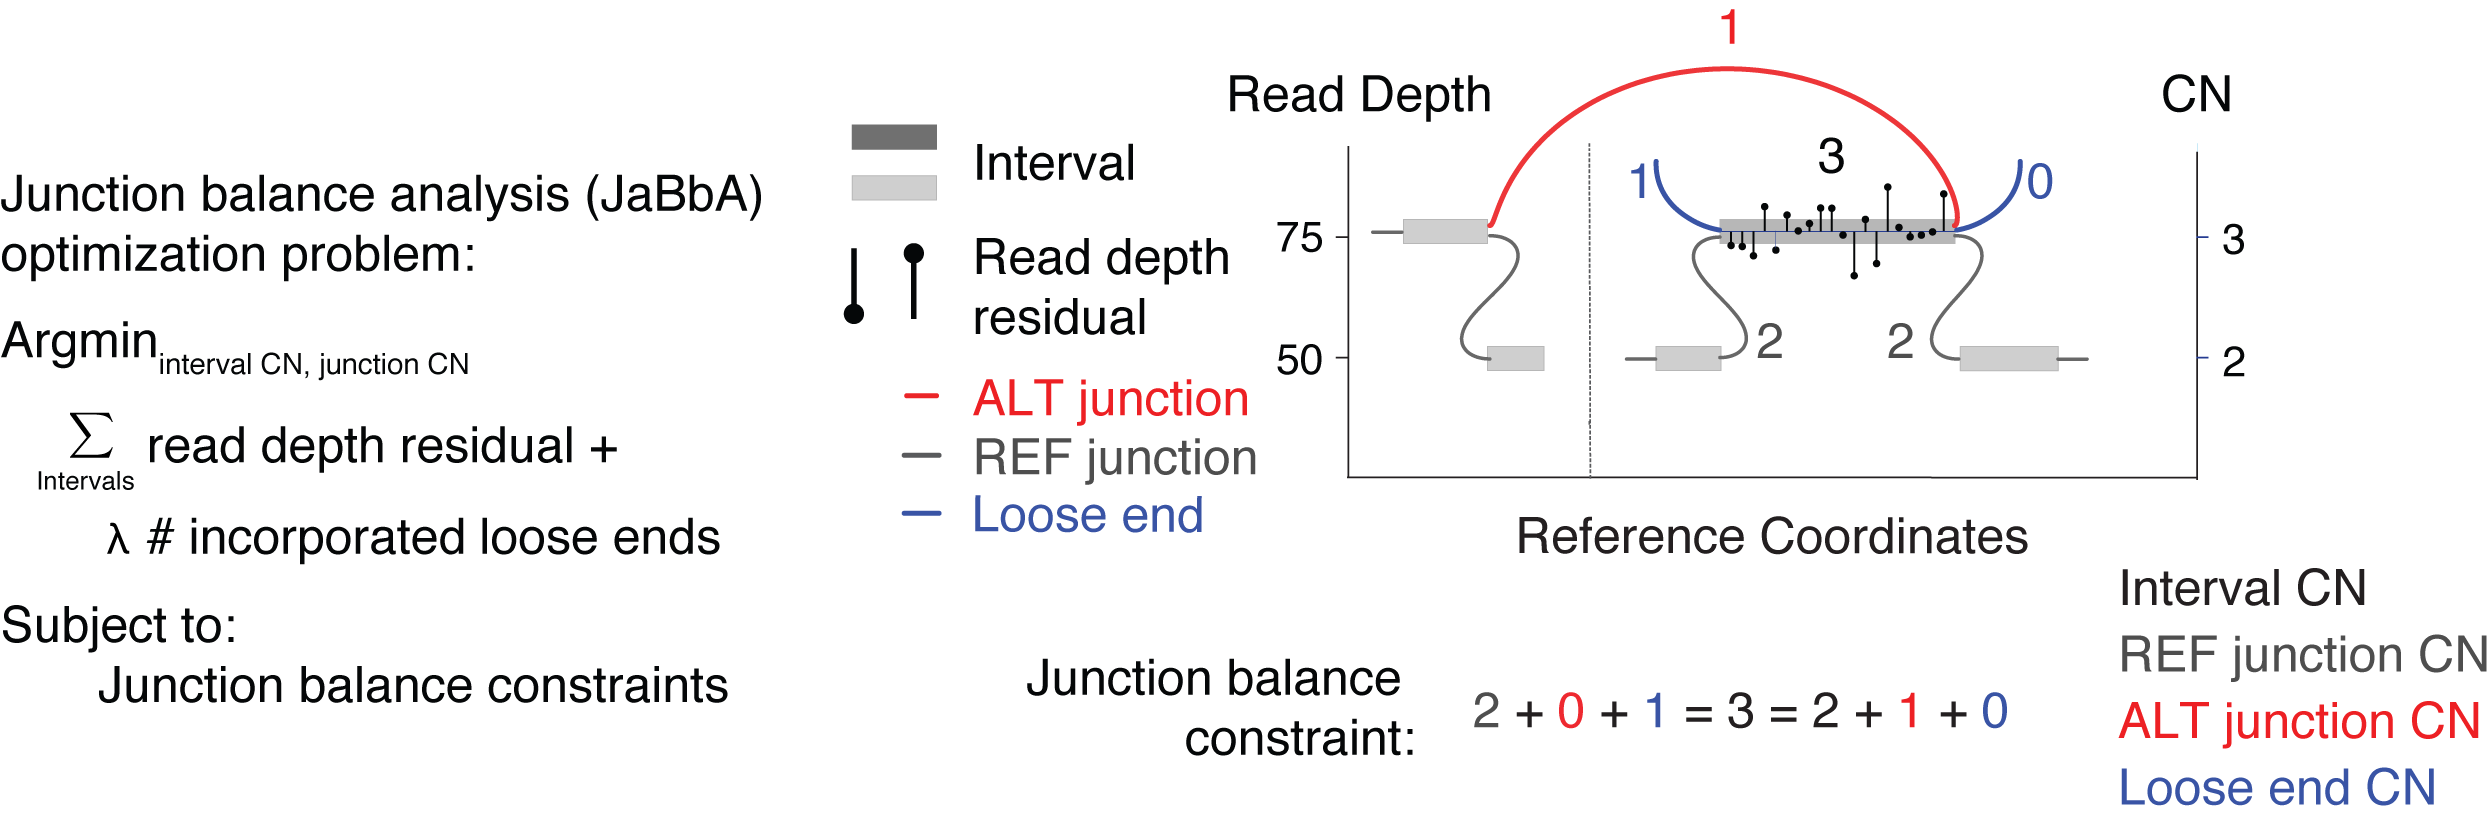
\includegraphics[width=0.95\linewidth]{figures/600ppi/jabba_formulation.png}
    \caption{\textbf{Formulation of Junction Balance Analysis} xxxx...}
    \label{fig:jabba_formulation}
\end{figure*}

We developed an algorithm, JaBbA, to infer junction-balanced genome graphs with high fidelity. Analogous to previous approaches, we define a (directed) genome graph of vertices representing strands of genomic segments and edges  representing a pair of 3' and 5' DNA ends that are adjacent in the reference genome (REF edge) or connected through rearrangement (ALT edge). A \textit{junction balanced genome-graph} assigns every vertex and edge in the graph an integer CN, while enforcing the constraint that the dosage of every interval (vertex) is equal to the sum of the JCN of the incoming (or similarly, outgoing) junctions (\textbf{Fig. \ref{fig:jabba_formulation}}).  The MIP optimization solved by JaBbA minimizes the residual between observed read depth and inferred interval dosage through joint assignment of CN to intervals and junctions (\textbf{Fig. {fig:Fig1}B, Fig. {fig:S1}C}, sec:methods).

\subsection{JaBbA pipeline}
Junction Balance Analysis (JaBbA, \url{https://github.com/mskilab/JaBbA}) is an R package freely available under the MIT license. The required inputs to JaBbA are binned (e.g. 200bp) and normalized read depth data $y$, purity $\alpha$, ploidy $\tau$, a set of junctions $\mathcal{A}$ (see mathematical formulation above), and a hyperparameter $\lambda$. The key output is a \texttt{gGraph} object representing a junction-balanced genome graph (i.e. solution to \textbf{Eq. \ref{eq:MIQP}}) which can be queried and analyzed using downstream algorithms, e.g. SV event classification algorithms in the \texttt{gGnome} package (\url{https://github.com/mskilab/gGnome}, see "Structural variant event classification" section below). The workflow of JaBbA is composed of four phases: read depth preprocessing, graph building, JaBbA model fitting, and postprocessing.

\subsubsection*{Data preprocessing}

\subsubsection*{Graph partitioning}

% \section{Automatic tuning of convergence criteria to improve the performance of harder problems}

\subsubsection*{Post processing and allelic CN fitting}

\section{JaBbA robustly produce accurate copy numbers for DNA segments and junctions}
JaBbA differs primarily from previous genome graph methods in its robust modeling of WGS read depth noise and explicit accounting of false negative junctions, also called loose ends (see \nameref{sec:methods}). In our benchmarking experiments, JaBbA inferred JCN with consistently higher fidelity than published genome graph-based methods (ReMixT \cite{McPherson2017-ry}, Weaver \cite{Li2016-qa}, PREGO \cite{Oesper2012-vw}) across a wide range of tumor purities (\textbf{Fig. \ref{fig:S1}D-E}). In addition, JaBbA qualitatively outperformed genome graph-based methods and even classic (i.e. non-graph based) CNA callers (BIC-seq \cite{Xi2011-oa} and CONSERTING \cite{Chen2015-sw}) in estimating interval CN and change point locations across a wide range of tumor purities (\textbf{Fig. \ref{fig:S1}F-I}). These results show that JaBbA is the first genome graph SV caller to accurately infer the topology of JCN while approaching (or exceeding) the fidelity of classic CNA callers. 

We also validated JaBbA's estimates of JCN from short-read WGS with 10X Chromium linked-read WGS, which provides a more direct readout of JCN with its high number of long junction-spanning fragments. In the breast cancer cell line HCC1954, JaBbA-derived JCN estimates closely correlated with the coverage of junction-spanning linked-read barcodes ($R^2 = 0.91$, \textbf{Fig. \ref{fig:Fig1}C}). This included examples of low JCN (e.g. JCN = 1) junctions connecting both low and high CN intervals, as well as high JCN (JCN = 10)  junctions (\textbf{Fig. \ref{fig:Fig1}D}). These results show that JCN is a property that can be robustly inferred from short-read WGS and is independent from (interval) CN. 

\section{Interactive visualization of genome graphs in arbitrary genomic windows}


\section{Discussion}

%%%%%%%%%%%%%%%%%%%%%%%%%%%%%%%%%%%%%%%%%%%%%%%
%% Chapter 3: discovery of novel SV patterns
%%%%%%%%%%%%%%%%%%%%%%%%%%%%%%%%%%%%%%%%%%%%%%%
\chapter{Distinct Classes of Complex Structural Variation Uncovered across Thousands of Cancer Genome Graphs}
In this chapter I will describe the discovery of three distinct types of complex SV events from 2778 genome graphs built with JaBbA from a pan-cancer cohort of over 30 types of cancers. Furthermore, I will show that the patients in this cohort can be stratified based on 13 simple to complex rearrangement patterns to clusters of differential overall survival, tumor type enrichment, and association with specific germline or somatic alterations.

\section{Analysis of pan-cancer genome graphs}
To investigate the topology of JCN across cancers, we assembled a dataset comprising 2,813 short-read WGS tumor or cell line samples spanning 31 primary tumor types (Table \ref{tab:S1}), including WGS for 539 previously unpublished cases  (\textbf{Table \ref{tab:S2}}). In total, our analysis included 1,648 WGS samples not included in the Pan-Cancer Analysis of Whole Genomes (PCAWG) effort \cite{pcawg_marker2020-yi}.  Application of harmonized pipelines followed by JaBbA (\textbf{Fig. \ref{fig:Fig1}B}) yielded 2,778 high quality genome graphs (\textbf{Fig. \ref{fig:Fig1}E}, see \nameref{sec:methods} for sample characteristics and exclusion criteria). 

% TODO: fix the table insertion
% \begin{table}[!ht]
%     \captionsetup{justification=raggedright,singlelinecheck=off}
%     \caption{\textbf{Pan-cancer WGS cohort summary, related to Figure \ref{fig:Fig1}} Summary (table in pdf format) of the number of samples from each tumor type and the number of cell line samples of a tumor type.}
%     \label{tab:S1}
% \end{table}

% \begin{table}[!ht]
%     \captionsetup{justification=raggedright,singlelinecheck=off}
%     \caption{\textbf{Sources of pan-cancer WGS datasets used in this study, related to Figure \ref{fig:Fig1}} Summary (table in pdf format) of the number of samples from each dataset, the completeness of the pipelines, and the citation if the dataset is published before.}
%     \label{tab:S2}
% \end{table}

Analyzing junction-balanced genome graph topology, we identified subgraphs associated with previously identified complex rearrangement patterns such as chromothripsis, chromoplexy, and TICs (\textbf{Fig. \ref{fig:Fig1}B, right panel}) implementing criteria described in previous publications within our framework (see \nameref{sec:methods}). Consistent with our 10X Chromium WGS benchmarks (see above) (\textbf{Fig. \ref{fig:Fig1}C}), we observed wide variation in inferred JCN across our datasets which correlated with observed read depth changes at breakends (\textbf{Fig. \ref{fig:Fig1}F}). While the vast majority of junctions demonstrated low-JCN (JCN $\leq$ 3), we observed a long tail of junctions with elevated– (JCN > 3) and high-JCN (JCN > 7) (\textbf{Fig. \ref{fig:Fig1}G}).

\section{Low JCN clusters of deletion-like and duplication-like junctions form rigma and pyrgo}
To distinguish between complex SV patterns associated with low-JCN vs. high-JCN junctions, we identified junction clusters based on their overlapping footprints on the reference and labeled each cluster as high- / low- JCN on the basis of its highest copy junction (high-JCN thresholded at $>$ 7). Considering clusters harboring three or more junctions, we found low-JCN clusters were significantly more likely to be dominated ($>$ 90\% representation of that type) by DEL-like ($P < \SI{2.2e-16}{}$, z-test, logistic regression) or DUP-like junctions ($P < \SI{2.2e-16}{}$) (\textbf{Fig. \ref{fig:S2}A}).

To rigorously nominate clusters of low copy DUP-like and DEL-like junctions within each tumor sample, we identified genomic tiles (1 Mbp width, 500 kbp stride) enriched in low-JCN of a given type (e.g. DEL-like) relative to a calibrated gamma-Poisson background model (see \nameref{sec:methods}). In each analysis, non-outlier tiles harbored apparent simple deletions or duplications (\textbf{Fig. \ref{fig:Fig2}A-B}). In contrast, outlier bins in the DUP-like model resembled "towers" of low-JCN DUP-like junctions  (\textbf{Fig. \ref{fig:Fig2}A, top right}) that we named \textit{pyrgo} (\textgreek{p'urgos}, Greek meaning tower). Outlier loci in the DEL-like models comprised subgraphs of interval CN "chasms" flanked by low-JCN DEL-like junctions whose interval CN often reached 0 (\textbf{Fig. \ref{fig:Fig2}B, top left}).  We named these patterns \textit{rigma} (ρήγμα, Greek meaning rift).

\section{Tyfonas is massively rearranged amplicon associated with elevated number of fusion genes}
We then sought to investigate the rearrangement patterns associated with high-JCN junctions (JCN $>$ 7) in our genome graphs.  \textit{A priori}, a junction at such an extreme of JCN may evolve through a double minute, BFBC, or an as yet undescribed mechanism for duplicating already rearranged DNA. To characterize classes of  amplification events associated with these high-JCN junctions, we first identified 12,588 subgraphs harboring an interval CN of at least twice ploidy among the 2,487 unique genome graphs (by patient) (\textbf{Fig. \ref{fig:Figure4}A}), then identified among these amplicons (amplified clusters within a genome) those that harbor at least one junction with JCN $>$ 7.  We annotated the resulting 1,703 high-JCN amplicons according to several features: 1) the maximum JCN normalized by the maximal interval CN, 2) the summed JCN associated with fold back inversion junctions (INV-like junctions that terminate and begin at nearly the same location in the genome) relative to the maximal interval CN, and 3) the number of junctions with elevated JCN (JCN>3) (see \nameref{sec:methods}).

Clustering and classification of amplicons (\textbf{Fig. \ref{fig:Figure4}B}) on the basis of these three features yielded three stable clusters (\textbf{Fig. \ref{fig:S4}A-B}) (see \nameref{sec:methods}).  Upon visual inspection, the first group, harboring low fold-back JCN but high maximal JCN, contained amplicons comprising a single high-JCN junction forming a high CN circular path in the graph (\textbf{Fig. \ref{fig:Figure4}C}) as well as more complex cyclic patterns spanning multiple discontiguous loci, consistent with a double minute.  The second group, demonstrating high fold-back JCN ($>$ 0.5), a low burden of elevated-JCN junctions ($<$ 26), and a "stair step" pattern of copy gains, was consistent with a BFBC (\textbf{Fig. \ref{fig:Figure4}D}) \cite{Zakov:2013cm}. The third group contained both high fold-back JCN ($\geq$0.50) and a significant burden of elevated JCN junctions ($\geq$26).  Upon visual inspection, these amplicons comprised dense webs of elevated  JCN junctions across subgraphs compris $>$ 100 Mbp of genomic material and often reaching CNs higher than 50 (\textbf{Fig. \ref{fig:S4}C}).  We dubbed these extremely large amplicons, which did not fit in previously defined categories, \textit{tyfonas} (τύφωνας, Greek meaning typhoon) (\textbf{Fig. \ref{fig:Figure4}E}).

\section{Clusters of pan-cancer patients based on SV event burdens show differential prognosis and is associated with tumor types and genetic backgrounds}
Tallying normalized junction counts across 13 event categories and 2,487 patients, we found 14 stable clusters using standard model selection metrics (\textbf{Fig. \ref{fig:Fig_cluster}A, Fig. \ref{fig:S7}A-B, Table \ref{tab:S3}}). Most clusters were dominated by 1-3 event types (e.g. CT = chromothripsis, BR = BFBC, rigma, DDT = deletion, duplication, TIC) with the exception of two: QUIET (few events) and SPRS (sparse, miscellaneous events).

Consistent with previous reports, the CT cluster was significantly enriched in prostate adenocarcinoma  (PRAD, $P = \SI{2.05e-5}{}$, $OR = 1.99$, single-sided z-test, Bayesian logistic regression, \cite{Kovtun2015-kq}) and glioblastoma multiforme (GBM, $P = \SI{5.00e-8}{}$, $OR = 2.61$, \cite{Furgason2015-rv})  (\textbf{Fig. \ref{fig:Fig_cluster}B}). Similarly, the CP (chromoplexy) cluster was significantly enriched in PRAD ($P = \SI{2.32e-10}{}$, $OR = 3.18$, \cite{baca2013}). DDT tumors (defined by high burdens of deletions, duplications, and templated insertion chains) were enriched in triple-negative breast cancer (TNBC) ($P < \SI{2.2e-16}{}$, $OR = 8.80$),  ovarian cancers ($P = \SI{7.03e-16}{}$, $OR = 6.89$), and more broadly sex-hormone driven tumors ($P = \SI{3.18e-14}{}$, $OR = 19.0$). 

Inspection of the heatmap in \textbf{Fig. \ref{fig:Fig_cluster}A} showed that the classes of complex SV introduced in this study (pyrgo, rigma, tyfonas) largely clustered independently from known complex SV types (double minute, BFBC, chromothripsis, chromoplexy). Among these, the BR (BFBC and Rigma dominated) cluster was primarily (60\%) composed of ESAD cases ($P < \SI{2.2e-16}{}$, $OR = 6.08$) and enriched in gastrointestinal tumors (e.g. esophageal, colorectal, and gastric adenocarcinoma) ($P < \SI{2.2e-16}{}$, $OR = 4.56$) (\textbf{Fig. \ref{fig:Fig_cluster}B}).  The TYF (tyfonas dominated) cluster was enriched in both luminal breast cancer ($P = \SI{4.87e-8}{}$, $OR = 3.25$),  HER2+ breast cancer ($P < \SI{2.64e-9}{}$, $OR = 4.96$), dedifferentiated liposarcoma ($P < \SI{2.2e-16}{}$, $OR = 24.5$), and acral melanoma ($P < \SI{1.84e-15}{}$, $OR = 7.40$). In contrast, cutaneous melanomas were enriched in the CT cluster.  Additional associations are shown in \textbf{Fig. \ref{fig:S7}C} and \textbf{Table \ref{tab:S6}}.

We associated somatic or constitutional genotypes in CGC genes with cluster membership, after correcting for tumor subtype as a covariate. More than 20\% of cases in the DDT cluster harbored constitutional ($P = \SI{1.60e-4}{}$, $OR = 3.81$) loss of function lesions in \textit{BRCA1} (\textbf{Fig. \ref{fig:Fig_cluster}C}). BR-cluster tumors were also significantly enriched in somatic \textit{TP53} mutations ($P < \SI{4.71e-7}{}$, $OR = 2.06$). Additional somatic genotype associations (\textbf{Fig. \ref{fig:S7}D}), included an enrichment of \textit{SMC4} ($P = \SI{2.33e-3}{}$, $OR = 3.11$) and \textit{RAD21} ($P = \SI{1.96e-3}{}$, $OR = 3.27$) mutations in the INVD (inverted duplication dominant) cluster, \textit{ARID1A} ($P = \SI{1.21e-3}{}$, $OR = 1.86$) mutations in the TIC (templated insertion chain dominant) cluster, and \textit{KMT2C} ($P = \SI{2.89e-3}{}$, $OR = 1.95$) mutations in the TRA (translocation-dominated) cluster.

Kaplan-Meier analysis revealed poor survival among novel SV-class dominated clusters (BR, PYR, and TYF) (\textbf{Fig. \ref{fig:Fig_cluster}D}, FDR $<$ 0.1, log rank test) as well as several clusters dominated by previously-described SV classes (CP, CT, and INVD) (\textbf{Fig. \ref{fig:S7}E}).  These effects persisted after correcting for clinical and molecular covariates in a Cox regression analysis, with BR ($P = \SI{1.17e-2}{}$, $HR = 1.72$, likelihood ratio test, Cox regression), PYR ($P = \SI{6.13e-3}{}$, $HR = 2.01$), TYF ($P = \SI{5.37e-3}{}$, $HR = 2.12$ , CP ($P = \SI{1.76e-3}{}; HR = 1.91$), CT ($P = \SI{6.69e-4}{}; HR = 1.83$), and INVD ($P = \SI{8.79e-4}{}; HR = 2.06$) clusters each demonstrating reduced survival relative to the QUIET cluster (\textbf{Fig. \ref{fig:Fig_cluster}E}, \textbf{Fig. \ref{fig:S7}F}).

\section{Discussion}


%%%%%%%%%%%%%%%%%%%%%%%%%%%%%%%%%%%%%%%%%%%%%%%
%% Chapter 4: SV evolution after telomere crisis
%%%%%%%%%%%%%%%%%%%%%%%%%%%%%%%%%%%%%%%%%%%%%%%
\chapter{Structural variant evolution after telomere crisis}
In this chapter I set out to capture the SV events in human cell lines directly resulting from natural telomere crisis

\section{Both simple and complex SVs detected in previously described post-crisis cell lines}

\section{An \textit{in vitro} model of natural telomere crisis in human lung fibroblast cell line MRC5}

\section{Screening for structural alterations in post-crisis MRC5 clones using low-pass WGS}

\section{Integrate SVs and SNVs to Reconstruct phylogeny of post-crisis clones with high-pass WGS}

\section{One allele of chromosome 12p with the shortest telomere length is the origin of genome instability during telomere crisis}

\section{Discussion}

%%%%%%%%%%%%%%%%%%%%%%%%%%%%%%%%%%%%%%%%%%%%%%%
%% Chapter 5: Whole genome analysis of RPA- lung adenocarcinoma
%%%%%%%%%%%%%%%%%%%%%%%%%%%%%%%%%%%%%%%%%%%%%%%
\chapter{Whole-genome characterization of lung adenocarcinomas lacking alterations in the RTK/RAS/RAF pathway}

In this final chapter, I describe the collaborative effort within the Cancer Genome Atlas (TCGA) consortium to characterize the whole genomes of lung adenocarcinoma lacking canonical pathogenic alterations in RTK/RAS/RAF pathway as determined by whole exome sequencing (WES) and transcriptome sequencing (RNA-seq).

\section{Introduction}
Lung adenocarcinoma (LUAD) is the most common lung malignancy and a leading cause of cancer death in the United States (Siegel et al., 2019). Most LUADs are driven by constitutive activation of MAPK signaling, which is, in turn, a consequence of alterations in receptor tyrosine kinases (RTK), downstream RAS/RAF/MEK cascade proteins, and their regulators (Desai et al., 2014). Comprehensive studies using whole-exome (WES) and/or transcriptome sequencing (RNA-seq) have identified RTK/RAS/RAF pathway driver alterations in 70-80\% of LUADs (Campbell et al., 2016; Cancer Genome Atlas Research Network, 2014; Imielinski et al., 2012). Because driver alterations in RTK/RAS/RAF pathway genes such as EGFR, BRAF, ALK, RET, ROS1, and KRAS, can be targeted by small molecule inhibitors that significantly prolong survival, therapeutic decision making in LUADs is routinely directed by testing for many, but not all RTK/RAS/RAF alterations to direct (Herbst et al., 2018).  

The remaining 20-30\% of cases, which we refer to as RTK/RAS/RAF pathway alteration-negative or RPA(-) LUADs, pose a major clinical challenge in precision thoracic oncology (Campbell et al., 2016). A key question is whether these RPA(-) LUADs represent a distinct RTK/RAS/RAF-independent entity that is associated with a unique evolutionary path and therapeutic sensitivities, or whether they have been mislabeled as RPA(-) due to technical factors (e.g., sample quality or limitations in the genomic profiling technologies). Specifically, apparent RPA(-) LUADs may harbor pathogenic variants in RTK/RAS/RAF pathway genes that are not adequately detected by WES, RNA-seq, or targeted gene panels such as those commonly used in large research studies or in clinical laboratories (Vinagre et al., 2013; Weischenfeldt et al., 2017).

We postulated that a more comprehensive analysis of candidate RPA(-) LUADs using whole-genome sequencing (WGS) in addition to WES and RNA-seq might illuminate more precisely the basic biology and also influence clinical management. We, therefore, performed WGS on LUAD samples from The Cancer Genome Atlas (TCGA) cohort that had appeared in previous analyses to lack an RTK/RAS/RAF pathway-activating alteration (Campbell et al., 2016). Since WGS is particularly effective in the identification of non-coding and structural genomic alterations, we hypothesized that analysis of those types of genome variation might reveal key features of RPA(-) LUAD biology.

\appendix
\chapter{Appendix A: Chapter \ref{chap:2} Supplementary materials and methods}


\bibliography{sampleThesis}

\end{document}